\chapter{NOISE ANALYSIS IN PULSE-PROCESSING DISCRETE-TIME FILTERS\footnotemark}
\label{chapter:theoretical}
\section{Introduction}
\footnotetext{See also \citep{avila101}.}
In particle physics experiments, where the results from the collisions are inferred from the measurement of electric charge in various sets of detectors \citep{gatti101,radeka101}, noise sets a fundamental limit for the charge measurement resolution \citep{degeronimo102}. In such experiments, the typical detector \mbox{front-end} circuit comprises a \mbox{charge-sensitive} amplifier (CSA) and a filter, often referred to as pulse shaper. The former is used to convert the input charge signal, coming from the detector electrodes, into a voltage signal, and is responsible for most of the noise present in the readout circuit signal path \citep{degeronimo101,degeronimo102}. The filter is used to convert the voltage signal at the CSA output into a shaped voltage pulse, in order to maximize the \mbox{signal-to-noise} ratio (SNR) at the measurement time.

Different noise analysis methods have been proposed to guide a proper filter design. The outcome of these methods is the equivalent noise charge ($\mathit{ENC}$), a measure of the \mbox{front-end} noise defined as the charge required at the detector input to produce an output SNR  of $1$. A \mbox{time-domain} analysis based on the weighting function (WF) concept \citep{radeka101, goulding101} has long been the preferred analysis, since it allows to find the optimum filter for a wide range of detector configurations \citep{radeka104,geraci101, gatti102,pullia103,pullia105}.

Traditionally, the filter synthesis has been performed using \mbox{continuous-time} networks. However, since producing arbitrary WFs by means of \mbox{continuous-time} analog circuitry is often impossible \citep{gatti102}, this approach does not always allow to synthesize optimum filters. A different approach based on \mbox{discrete-time} filters, implemented by means of digital signal processor (DSP) units \citep{geraci103,sampietro101,jordanov101} or switched capacitor networks \citep{porro101,fiorini101,abusleme101}, allows to synthesize WFs with virtually any shape, producing \mbox{near-optimum} filters. Moreover, this promising approach takes advantage of the aggressive technology scaling and the new techniques of the \textsc{vlsi} industry, allowing to implement fast, reliable and flexible filters.

In this work, a mathematical framework for a \mbox{design-oriented} analysis of \mbox{discrete-time} filters in the \mbox{discrete-time} domain is presented. Although \mbox{discrete-time} filters can be analyzed using a \mbox{continuous-time} method, it is not insightful and the resulting expressions are complex and difficult to use for design purposes. Furthermore, the analysis of \mbox{discrete-time} filters in the \mbox{discrete-time} domain provides a better insight on how their discrete nature affects the \mbox{front-end} noise. The proposed analysis can produce \mbox{closed-form} expressions for the $\mathit{ENC}$ calculation, which can be used for efficient algorithms for the $\mathit{ENC}$ evaluation and filter optimization procedures.

In order to validate the proposed framework in this work, an example is developed, and the result obtained is analyzed and compared with the result provided by the \mbox{continuous-time} approach. Also, an example of optimal filter computation is presented to demonstrate the capabilities of the proposed framework.


%%%%%%%%%%%%%%%%%%%%%%%%%%%%%%%%%%%%%%%%%%%%%%%%%%%%%%%%%%%%%%%%%%%%%%%%%%%%%%
%%%%%%%%%%% SECTION II: DISCRETE-TIME ANALYSIS %%%%%%%%%%%%%%%%%%%%%%%%%%%%%%%
%%%%%%%%%%%%%%%%%%%%%%%%%%%%%%%%%%%%%%%%%%%%%%%%%%%%%%%%%%%%%%%%%%%%%%%%%%%%%%
\section{Discrete-Time Analysis}

\figurename~\ref{fig:system} shows a simplified model to compute the \mbox{output-referred} noise contribution of a single noise source in a typical \mbox{front-end} detector. It consists of a linear block with a transfer function $H(s)$ that models the effect of the CSA on the noise source under analysis, and a \mbox{pulse shaper}, which in this case is a finite impulse response (FIR) filter with a \mbox{discrete-time} transfer function given by
\begin{equation}
F(z) = \sum_{j=0}^{N-1}a_{N-j} \hspace{0.1em}z^{-j} \label{eq:FIRtf}
\end{equation}
where $a_{N-j}$ are arbitrary coefficients and $N$ is the filter length. The noise source is characterized by its \mbox{two-sided} power spectral density (PSD) $\overline{n^2}(f)$.

For this analysis it is not necessary to consider the details of the physical processes that cause the noise. It will be assumed that the noise source is an arbitrary white or filtered white noise source, which represents any of the fundamental noise sources present at a detector front-end circuit, such as thermal noise, shot noise and flicker noise. This assumption allows to model the noise source in the time domain in terms of a sequence of noise pulses with core function $y(t)$, arriving Poissonianly at times $t_a$ with an average rate $\nu$ and random sign \citep{radeka101, goulding101}. A general procedure to calculate a function $y(t)$ that represents the noise process characterized by $\overline{n^2}(f)$ can be found in \citep{pullia102}.

By using the CSA transfer function and $y(t)$, the effect of an individual noise pulse at the filter input can be determined as
\begin{equation}
\hat{y}(t) = y(t) \ast \mathcal{L}^{-1}\!\left\{ H(s)\right\}\hspace{-0.15em}(t).\label{eq:shaped-pulse}
\end{equation}
Both sequences of pulses, at the input and at the output of $H(s)$, are illustrated in \figurename~\ref{fig:system}.

\begin{figure}[!t]
	\centering
	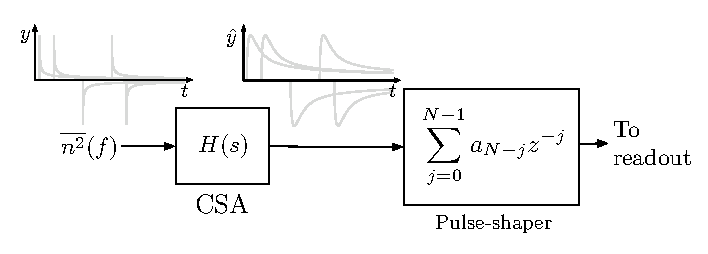
\includegraphics[width=4in]{./Figures/system.eps}
	\caption{Model for noise analysis in a typical \mbox{front-end} circuit.}\label{fig:system}
\end{figure}

Assuming a periodic, synchronous \mbox{front-end}, where the stimulus arrival time within each frame is fixed and known, the CSA can be reset at the beginning of each frame, prior to the corresponding stimulus. Thus, the analysis can be carried out considering a non-stationary noise process that starts at $t=0$. Then the total integrated noise at the filter input is a function of time \citep{radeka201}. Using \eqref{eq:shaped-pulse} and Campbell's theorem, the following expression for the total integrated noise at the filter input can be derived:
\begin{equation}
\sigma^2(t) = \nu\hspace{-.25em}\int_{0}^{t}\hspace{-.45em}\hat {y}^2(t-t_a)\;\mathrm{d}t_a\label{eq:envelope}.
\end{equation}

Let us define $P_i$ as the time interval between an arbitrary sample $i$ and its predecessor, given by $P_i=[(i-1)T_s, iT_s]$, where $T_s$ is the filter sampling period. Now consider the noise contribution of the pulses originated within $P_i$ and measured at an arbitrary sample $k$ (i.e., $t=kT_s$), $\sigma_i^2(k)$, as shown in \figurename~\ref{fig:sequence}. Using Campbell's theorem,  $\sigma_i^2(k)$ can be computed as
\begin{equation}
\sigma_i^2(k) = \nu\hspace{-.25em} \int_{(i-1)T_s}^{iT_s} \hspace{-.15em}  \hat{y}^2(kT_s-t_a)\;\mathrm{d}t_a\hspace{0.1em}. \label{eq:int2}
\end{equation}
It can be shown that \eqref{eq:int2}, can be expressed as
\begin{equation}
		\sigma_i^2(k) = \int_{0}^{T_s} \hspace{-.45em} \hat{y}^2\left(\left(k-i+1\right)T_s-\eta_1\right)\; \mathrm{d}\eta_1 
		\label{eq:ap1}
\end{equation}
where $\eta_1 = t_a+T_s-iT_s$. This integral can be split into two integrals as follows
\begin{eqnarray}
		\sigma_i^2(k) \hspace{-0.6em} &=& \hspace{-0.6em} \int_{0}^{(k-i+1)T_s} \hspace{-.65em} \hat{y}^2\left(\left(k-i+1\right)T_s-\eta_1\right)\; \mathrm{d}\eta_1 \nonumber\\
		&&\hspace{-0.8em}{-}\: \int_{T_s}^{(k-i+1)T_s} \hspace{-.65em} \hat{y}^2\left(\left(k-i+1\right)T_s-\eta_2\right)\; \mathrm{d}\eta_2.  
		\label{eq:ap2}
\end{eqnarray}
Defining $\eta_2 = \eta_3 + T_s$,~\eqref{eq:ap2} can be written as
\begin{eqnarray}
		\sigma_i^2(k) &=& \int_{0}^{(k-i+1)T_s} \hspace{-.45em} \hat{y}^2\left(\left(k-i+1\right)T_s-\eta_1\right)\; \mathrm{d}\eta_1 \nonumber\\
		&&{-}\: \int_{0}^{(k-i)T_s} \hspace{-.45em} \hat{y}^2\left(\left(k-i\right)T_s-\eta_3\right)\; \mathrm{d}\eta_3.  
		\label{eq:ap3}
\end{eqnarray}
Since $\hat{y}^2(t)$ is zero for negative arguments, then \mbox{$\sigma_i^2(k)= 0$} for $k < i$. For $k \geq i$, and according to~\eqref{eq:envelope},~\eqref{eq:ap3} can be alternatively expressed as
\begin{equation}
		\sigma_i^2(k) = \sigma^2\left(\left(k-i+1\right)T_s\right)-\sigma^2\left(\left(k-i\right)T_s\right) 
		\label{eq:ap4}
\end{equation}
therefore,
\begin{equation}
  \sigma_i^2(k) \hspace{-0.2em}=\hspace{-0.2em} 
  \begin{cases}
     \sigma^2((k-i+1)T_s)-\sigma^2((k-i)T_s ), & k \geq i   \\
      0, &   k < i.
  \end{cases}\label{eq:sigmaj}
\end{equation}

\begin{figure}[!t]
	\centering
	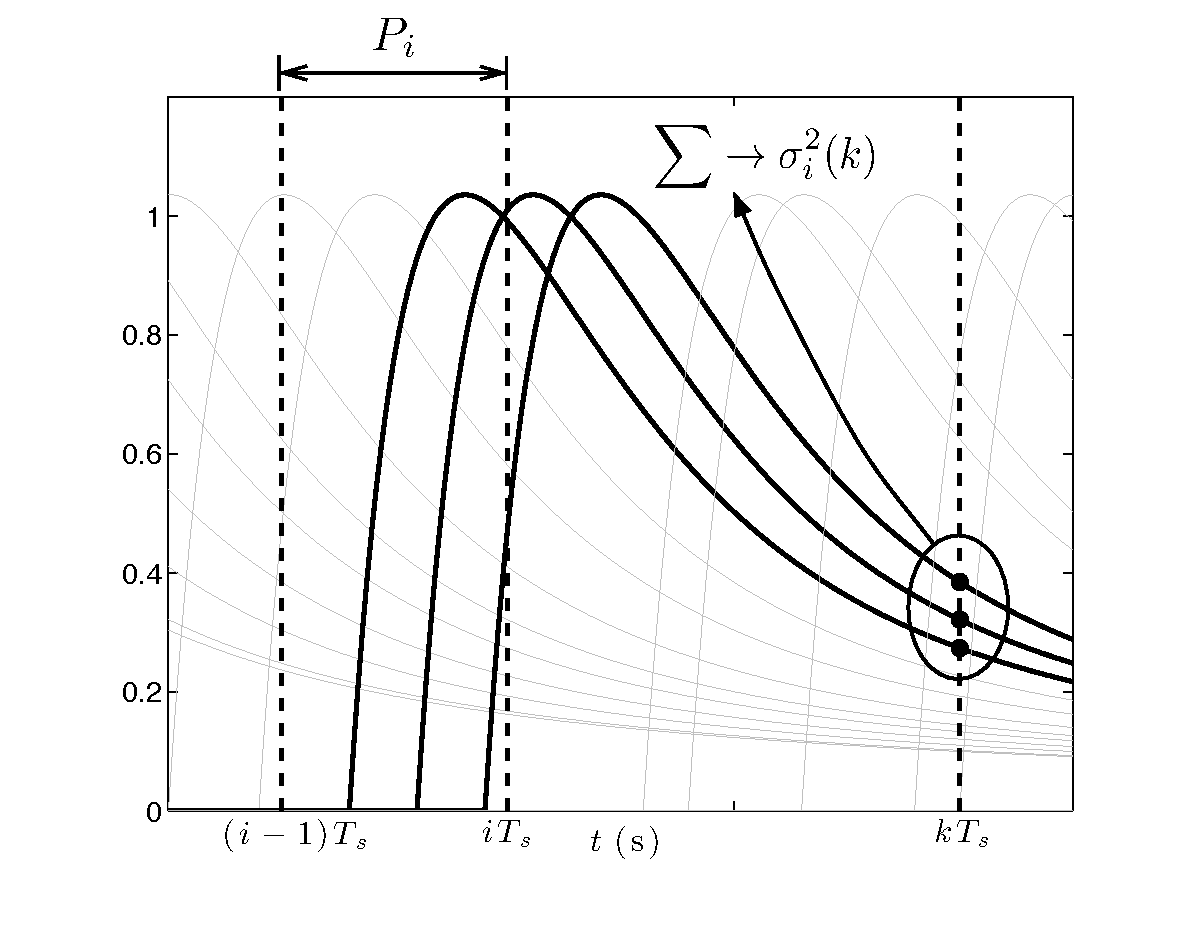
\includegraphics[width=4.5in]{./Figures/sequence.eps}
	\caption[Noise contribution of the pulses generated within $P_i$.]{Noise contribution of the pulses generated within $P_i$ and measured at an arbitrary sample $k$ (i.e., $t=kT_s$), using an arbitrary filtered noise core function $\hat{y}(t)$. The independent contribution of each pulse is pointed out with black dots.}\label{fig:sequence}
\end{figure}

Based on \eqref{eq:sigmaj}, the total integrated noise at the filter input measured at the \mbox{$k$-th} sample, $\sigma^2(kT_s)$, can be written as the sum of the individual noise contributions originated at each interval $P_i$:
\begin{equation}
\sigma^2(kT_s) = \sum_{i=1}^{N} \sigma_i^2(k). \label{eq:noise_evo}
\end{equation}
The evolution of the total integrated noise at the filter input according to \eqref{eq:noise_evo} is illustrated in \figurename~\ref{fig:envelope-example}. 

Since \eqref{eq:noise_evo} is composed by noise contributions originated at different time intervals $P_i$, the total integrated noise at the filter input holds partial correlation between samples, and the output noise cannot be computed by convolving \eqref{eq:noise_evo} with $F(z)$. However, since all evaluations of $\sigma_i^2(k)$ are originated from the same pulses (for a fixed $i$), and thus are fully correlated, \eqref{eq:noise_evo} can be split into $N$ independent \mbox{discrete-time} signals $\sigma_1^2(k), \sigma_2^2(k) \ldots \sigma_N^2(k)$. Each of these signals can be referred to the filter output as
\begin{align}
\hat{\sigma}_i(k) &= \sqrt{\sigma^2_i(k) } \ast \mathcal{Z}^{-1}\!\left\{ F(z) \right\}\hspace{-0.15em}(k) \nonumber \\
          &= \sum_{j=0}^{k-i} a_{N-j} \sqrt{\sigma^2_i(k-j)}.  \label{eq:sigmao}
\end{align}
Signals $\hat{\sigma}_1(k), \hat{\sigma}_2(k) \ldots \hat{\sigma}_N(k)$ are also independent, and can be added up as noise variances to compute the total integrated noise at the filter output as a function of $k$:
\begin{align}
\hat{\sigma}^2(k) &= \sum_{i=1}^k \hat{\sigma}_i^2(k) \nonumber \\
		       &= \sum_{i=1}^k \left(\sum_{j=0}^{k-i} a_{N-j}\sqrt{\sigma_i^2(k-j)}\right)^2 \hspace*{-7pt}.  \label{eq:sigmatk}
\end{align}
Evaluating \eqref{eq:sigmatk} at the measurement time \mbox{$t_m=NT_s$} \mbox{(i.e., $k=N$)} yields
\begin{align}
\hat{\sigma}^2(N) = \sum_{i=1}^N \left(\sum_{j=0}^{N-i} a_{N-j}\sqrt{\sigma_i^2(N-j)}\right)^2\hspace*{-7pt}.\hspace{0.2em} \label{eq:sigmaNprev}
\end{align}
Finally, replacing \eqref{eq:sigmaj} in \eqref{eq:sigmaNprev} and defining $h = N-j-i$, a closed-form expression for the front-end noise can be obtained:
\begin{equation}
\hat{\sigma}^2(N) = \sum_{i=1}^N \left( \sum_{h=0}^{N-i} a_{i+h} \sqrt{\sigma^2((h+1)T_s)-\sigma^2(hT_s)}\right)^2\hspace{-0.5em}. \label{eq:final}
\end{equation}

\begin{figure}[!t]
	\centering
	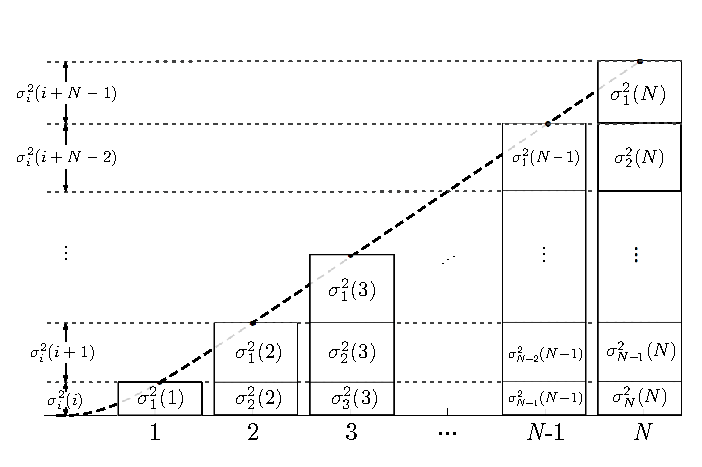
\includegraphics[width=5in]{./Figures/envelope-example.eps}
	\caption[Evolution of the total integrated noise at the filter input.]{Evolution of the total integrated noise at the filter input, where the noise of each sample was split according to \eqref{eq:noise_evo}.}\label{fig:envelope-example}
\end{figure}

The only term of \eqref{eq:final} that depends on the input-referred noise process is $\sigma^2(t)$, which can be calculated analytically or numerically for typical noise processes by using \eqref{eq:envelope}. For instance, \figurename~\ref{fig:envelopes} illustrates $\sigma^2(t)$ for thermal, shot and flicker noise. Even though the analysis presented here has been applied for a single noise source, it can be easily extended for circuits with several noise sources by applying the superposition principle in quadrature. 

\begin{figure}[!t]
	\centering
	\includegraphics[width=4.2in]{./Figures/envelopes.eps}
	\caption[$\sigma^2(t)$ for thermal, shot and flicker noise.]{$\sigma^2(t)$ for thermal, shot and flicker noise with normalized time $t/\tau$ and an arbitrary amplitude.}\label{fig:envelopes}
\end{figure}

%%%%%%%%%%%%%%%%%%%%%%%%%%%%%%%%%%%%%%%%%%%%%%%%%%%%%%%%%%%%%%%%%%%%%%%%%%%%%%
%%%%%%%%%%% SECTION III: EXAMPLE %%%%%%%%%%%%%%%%%%%%%%%%%%%%%%%%%%%%%%%%%%%%%
%%%%%%%%%%%%%%%%%%%%%%%%%%%%%%%%%%%%%%%%%%%%%%%%%%%%%%%%%%%%%%%%%%%%%%%%%%%%%%
\section{Example}
For validation purposes, the thermal noise contribution at the output of a \mbox{discrete-time} integrator filter will be computed using the proposed \mbox{discrete-time} analysis. The result obtained will be analyzed and then compared with the result produced by the traditional \mbox{continuous-time} approach. \figurename~\ref{fig:analysis-circuit} shows the front-end circuit used for general noise analysis. The detector is modeled as capacitance $C_D$, whereas the CSA is shown as a voltage amplifier with open loop gain $A(s) = A/(1+s\tau)$, input capacitance $C_{in}$ and a feedback capacitor $C_F$. Resistor $R_R$ across the feedback capacitor $C_F$ represents the CSA reset element. The filter coefficients are $a_i=1$. The detector shot noise represented by $\overline{i^2_D}$ will be omitted for the purpose of this example. Thermal noise has been assumed to be dominated by the CSA input device and is represented by two \mbox{fully-correlated} noise sources \citep{sansen101}, a voltage white noise source with a \mbox{two-sided} PSD $\overline{v_n^2}$ and a current noise source with a \mbox{two-sided} PSD $\overline{i_n^2}$. Both noise sources are related as follows:
\begin{equation} 
\overline{i_n^2} = (sC_{in})^2 \hspace{0.2em}\overline{v_n^2}\label{eq:current}.
\end{equation}

Considering that the effect of the reset switch during the relatively short time that it takes the CSA to produce an output voltage is negligible, $R_R$ can be assumed to be infinite \citep{pullia102}. The CSA open loop DC gain ($A$) is assumed to be very large as well. Under these assumptions and using \eqref{eq:current}, the PSD of the thermal noise referred to the CSA output, $\overline{v_o^2}$, can be approximated to
\begin{equation} 
	\overline{v_o^2} \approx \left|\frac{C_{tot}}{C_f} \frac{1}{1+s\hat{\tau}}\right|^2\overline{v_n^2} \label{eq:ex-PSD}
\end{equation}
where $C_{tot} = C_D+C_F+C_{in}$ and $\hat{\tau} = (\tau/A) (\hspace{0.2em}C_{tot}/C_f)$ is the CSA \mbox{closed-loop} \mbox{time-constant}.

\begin{figure}[!t]
	\centering
	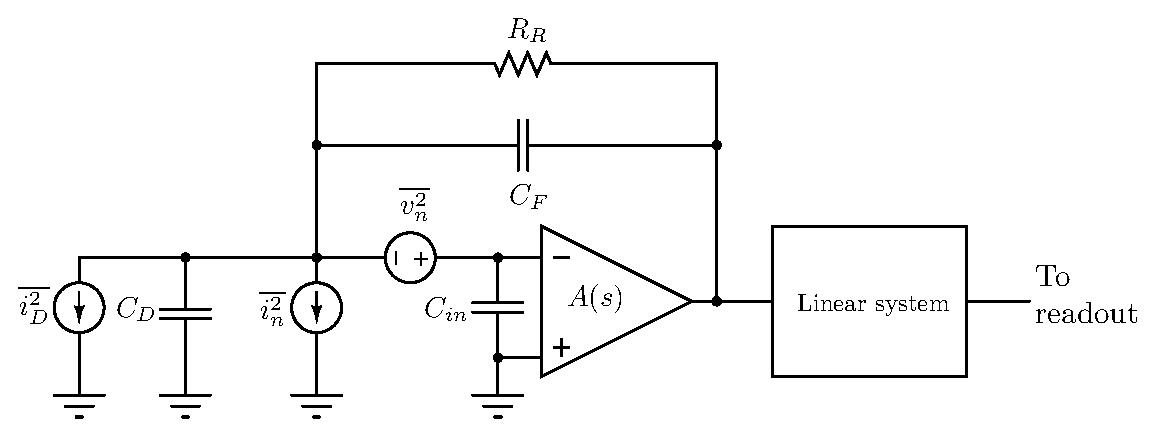
\includegraphics[width=5in]{./Figures/front-end.eps}
	\caption{Front-end circuit used for noise analysis.}\label{fig:analysis-circuit}
\end{figure}

The PSD in \eqref{eq:ex-PSD} can be treated as the result of passing a fictitious noise source with PSD $\overline{v_n^2}$ through a block with transfer function $H_\text{th}(s)$ given by
	\begin{equation} 
		H_\text{th}(s) =  \frac{C_{tot}}{C_f}\frac{1}{1+s\hat{\tau}}. \label{eq:exampletf}
	\end{equation}

Since $\overline{v_n^2}$ characterizes a white noise source, it can be modeled as a sequence of Dirac impulses with core function $y_\text{th}(t)$ occurring at an arbitrary rate $\nu$ and random sign \citep{pullia102}, where $y_\text{th}(t)$ is given by
	\begin{equation} 
		y_\text{th}(t) = \sqrt{\frac{\overline{v_n^2}}{\nu}}\delta(t)\label{eq:pulseW}.
	\end{equation}
Replacing \eqref{eq:exampletf} and \eqref{eq:pulseW} in \eqref{eq:shaped-pulse}, each pulse in the sequence can be referred to the CSA output as an exponentially decaying pulse \citep{pullia102} as follows
	\begin{equation} 
		\hat{y}_\text{th}(t-t_a)  = \sqrt{\frac{\overline{v_n^2}}{\nu}}\frac{C_{tot}}{C_F} \frac{ e^{-(t-t_a)/\hat{\tau}}}{\hat{\tau}}u(t-t_{a}) \label{eq:shapedW}
	\end{equation}
where $u(t)$ is the unit step function. Substituting \eqref{eq:shapedW} in \eqref{eq:envelope}, the filter input total integrated noise due to the thermal noise, $\sigma_\text{th}^2(t)$, can be derived:
	\begin{equation} 
		\sigma_\text{th}^2(t) = \overline{v_n^2} \frac{C_{tot}^2}{C_F^2}  \frac{1-e^{-2t/\hat{\tau}}}{2\hat{\tau}}u(t). \label{eq:envelopeW}
	\end{equation}
Finally, replacing \eqref{eq:envelopeW} in \eqref{eq:final} and defining $x=e^{T_s/\hat{\tau}}$, the front-end noise, $\hat{\sigma}_\text{th}^2(N)$, can be obtained:
	\begin{equation}
	\hat{\sigma}_\text{th}^2(N)  = \frac{\overline{v_n^2}}{2\hat{\tau}}\frac{C_{tot}^2}{C_F^2}\frac{\left(N(x^2\hspace{-0.1em}-\hspace{-0.1em}1) \hspace{-0.1em}-		\hspace{-0.1em}2x\hspace{-0.1em}-\hspace{-0.1em}x^{-{2N}}\hspace{-0.25em}+\hspace{-0.1em}2x^{-{N}}\hspace{-0.25em}+\hspace{-0.1em}2x^{1-N}		\hspace{-0.2em}-1 \right)}{(x-1)^2}\hspace{-2pt}.   \label{eq:exFinal}
	\end{equation}
	
When the time interval between samples is large enough to consider that consecutive noise samples are uncorrelated \mbox{(i.e., $\hat{\tau} \ll T_s$),} $\hat{\sigma}_\text{th}^2(N)$ can be approximated without the use of the proposed analysis as a weighted sum of the uncorrelated samples of the total integrated noise at the CSA output as follows:
\begin{equation}
	\left. \hat{\sigma}_\text{th}^2(N)\right\rvert_{\hat{\tau}\ll T_s}  \approx  N \lim_{t\rightarrow \infty} \sigma^2(t) = N \frac{\overline{v_n^2}}{2\hat{\tau}}\frac{C_{tot}^2}{C_F^2}. \label{eq:aprox}
\end{equation}

As shown in \figurename~\ref{fig:exampleSigma}, \eqref{eq:exFinal} behaves as predicted by \eqref{eq:aprox} for small values of $\hat{\tau}$.
\begin{figure}[!t]
	\centering
	\includegraphics[width=4in]{./Figures/example.eps}
	\caption{$\hat{\sigma}_\text{th}^2(N)$  and $N \frac{\overline{v_n^2}}{2\hat{\tau}}\frac{C_{tot}^2}{C_F^2}$ as a function of $\hat{\tau}$, using $\overline{v_n^2} = 1$, \mbox{$C_{tot}^2/C_F^2 = 1$} and $N = 20$.}\label{fig:exampleSigma}
\end{figure}

Now, the same example will be analyzed using the traditional \mbox{continuous-time} approach. Using \eqref{eq:shapedW}, the WF $w(t)$, defined as the contribution of each pulse occurring at time $t$ measured at a fixed time $t_m=NT_s$ at the output of the filter, is given by
\begin{align}
	w(t) &= \sum_{n=1}^{N} \hat{y}_\text{th}(nT_s-t) \nonumber \\
       	 &=\sqrt{\frac{\overline{v_n^2}}{\nu}} \frac{C_{tot}}{C_F}\sum_{n=1}^{N} \frac{e^{-(nT_s-t)/\hat{\tau}}}{\hat{\tau}} u(nT_s-t) \label{eq:WF}.
\end{align}
Integrating \eqref{eq:WF} from the reset time ($t=0$) to the signal measurement time ($t=t_m$), the filter total integrated noise at $t=t_m$ can be computed as
\begin{align} 
	\hat{\sigma}_\text{th}^2(N) &= \nu \hspace{-0.3em}\int_{0}^{t_m}\hspace{-0.5em}w^2(t)\,\text{d}t \nonumber \\
									&= \overline{v_n^2} \frac{C_{tot}^2}{C_F^2} \int_{0}^{NT_s} \hspace{-0.4em}\left(\sum_{n=1}^{N} \frac{e^{-(nT_s-t)/\hat{\tau}}}{\hat{\tau}} u(nT_s-t)\right)^{\hspace{-0.2em}2}\hspace{-0.4em}\text{d}t \label{eq:pre1}.
\end{align}
Defining $\alpha = T_s/\hat{\tau}$ and $\beta = t/\hat{\tau}$, \eqref{eq:pre1} can be \mbox{re-written} as
\begin{equation}
	\hat{\sigma}_\text{th}^2(N)   = \frac{\overline{v_n^2}}{\hat{\tau}}\frac{C_{tot}^2}{C_F^2}\int_{0}^{N\alpha}e^{2\beta} \left(\sum_{n=1}^{N}e^{-n\alpha}u\left(n\alpha-\beta\right) \right)^{\hspace{-0.3em}2}\hspace{-0.1em}\text{d}\beta \label{eq:pre2}
\end{equation}
which can be split into a sum of integrals as follows
\begin{equation}
	\hat{\sigma}_\text{th}^2(N) = \frac{\overline{v_n^2}}{\hat{\tau}}\frac{C_{tot}^2}{C_F^2}\sum_{n=1}^{N}\int_{(n-1)\alpha}^{n \alpha} e^{2\beta} \left(\sum_{k = n}^{N} e^{-k\alpha}\right)^{\hspace{-0.3em}2}\hspace{-0.1em}\text{d}\beta \label{eq:pre3}.
\end{equation}
Finally, defining $x= e^{\alpha}$ it can be shown that \eqref{eq:pre3} is equal to \eqref{eq:exFinal}.

%%%%%%%%%%%%%%%%%%%%%%%%%%%%%%%%%%%%%%%%%%%%%%%%%%%%%%%%%%%%%%%%%%%%%%%%%%%%%%
%%%%%%%%%%% SECTION IV: OPTIMIZATION %%%%%%%%%%%%%%%%%%%%%%%%%%%%%%%%%%%%%%%%%
%%%%%%%%%%%%%%%%%%%%%%%%%%%%%%%%%%%%%%%%%%%%%%%%%%%%%%%%%%%%%%%%%%%%%%%%%%%%%%
\section{$\mathit{ENC}$ Minimization}

For filter optimization purposes, a typical \mbox{front-end} circuit with thermal, shot and flicker noise components is considered. The \mbox{front-end} configuration from \figurename~\ref{fig:analysis-circuit} will be used. In this case, the pulse shaper is a \mbox{discrete-time} FIR filter with indeterminate coefficients $a_i$. Shot noise is assumed to be dominated by the detector noise and is represented by a white noise current source with \mbox{two-sided} PSD $\overline{i^2_D}$ in parallel with the detector capacitance $C_D$ and given by
	\begin{equation} 
		\overline{i^2_D} = qI_L
	\end{equation}
where $q$ is the electron charge and $I_L$ the detector leakage current. Thermal noise and flicker noise are assumed to be dominated by the noise of the CSA input device and are represented by two \mbox{fully-correlated} noise sources, a voltage noise source with \mbox{two-sided} PSD $\overline{v_n^2}$ given by
	\begin{equation} 
		\overline{v_n^2} =   a_T + \frac{a_F}{|f|}
	\end{equation}
where $a_T$ and $a_F$ are the thermal and flicker coefficients, and a current noise source with \mbox{two-side} PSD $\overline{i_n^2}$ given by \eqref{eq:current}. Traditionally, the coefficients $a_T$ and $a_F$ are obtained from the CSA input device models. However, for design purposes the most accurate values shall be used, and these coefficients should be extracted from experiments \citep{bertuccio101} or precise simulations.

Considering the contribution of each noise process separately, the $\mathit{ENC}^2$ for the output measured at $t = NT_s$ can be written as 
	\begin{equation}
		\mathit{ENC}^2 = \frac{\hat{\sigma}_\text{shot}^2(N)+\hat{\sigma}_\text{th}^2(N) +  \hat{\sigma}_{1/f}^2(N)}{q^2\left| \max[w(t)]		\right|^2/C_F^2}\label{eq:enc}
	\end{equation}
where $\hat{\sigma}_\text{shot}^2(N)$ is the shot noise contribution, $\hat{\sigma}_\text{th}^2(N)$ is the thermal noise contribution, $\hat{\sigma}_{1/f}^2(N)$ is the flicker noise contribution and $w(t)$ is the weighting function at the \mbox{front-end} output given by \eqref{eq:WF}.

In order to find the coefficients $a_i$ that minimize \eqref{eq:enc}, and hence the optimal FIR filter, the signal measurement time $t_m=NT_s$ was assumed to be a constant determined by the processing time budget constraints, and the filter sampling period $T_s$ was assumed to be a constant determined by the filter maximum clock rate. Although $\hat{\tau}$ is a design variable that depends on the CSA and not on the filter, it has been included in the optimization analysis. 

Given that a common WF reaches its maximum value at \mbox{$t=t_m/2$}, and that the WF height is commonly a design constraint, the denominator of \eqref{eq:enc} was forced to be constant by fixing the WF height, $h_{w}$, through the following constraints
	\begin{align}
		\sum_{i=1}^{N/2} a_{i}\left(1-e^{ - T_s(N/2-i+1)/\hat{\tau}}\right) &= h_w \label{eq:con1}\\
		\sum_{i=1}^{N} a_{i}\left(1-e^{-T_s(N-i+1)/\hat{\tau}}\right) &= 0 \label{eq:con2}.
	\end{align}
Although these constraints appear from foreknowledge about the shape of the optimum WF, the actual computation of $w(t)$ was never required for the optimization problem formulation. For illustration purposes, the length of the filter $N$ was assumed to be an even number. Considering these constraints, minimizing the $\mathit{ENC}^2$ is equivalent to minimizing its numerator, and according to \eqref{eq:final}, the resulting objective function $f_o$ is given by
	\begin{eqnarray} 
		f_o \hspace{-0.7em}&=  \hspace{-0.7em} &\sum_{i=1}^N \left\{\left( \sum_{h=0}^{N-i} a_{i+h} \sqrt{\sigma_\text{shot}^2((h+1)T_s)-\sigma_\text{shot}^2(hT_s)}\right)^{\hspace{-0.3em}2} \right.\nonumber\\
		\hspace{-1em}&  \hspace{-1em}&+ \left( \sum_{h=0}^{N-i} a_{i+h} \sqrt{\sigma_\text{th}^2((h+1)T_s)-\sigma_\text{th}^2(hT_s)}\right)^{\hspace{-0.3em}2} \nonumber\\
		\hspace{-1em}&  \hspace{-1em}& + \left.\left( \sum_{h=0}^{N-i} a_{i+h} \sqrt{\sigma_{1/f}^2((h+1)T_s)-\sigma_{1/f}^2(hT_s)}\right)^{\hspace{-0.3em}2} \right\} \nonumber. \\\label{eq:fo}
	\end{eqnarray}

To obtain a numerical solution for the optimization problem, given by the objective function \eqref{eq:fo} and constraints \eqref{eq:con1} and \eqref{eq:con2}, the parameters of an HPGe segmented detector with an input FET transistor were considered. Assuming that the input device is in strong inversion, the coefficient $a_T$ can be calculated as
	\begin{equation} 
		a_T = \frac{2 K T \gamma}{g_m}
	\end{equation}
where $K$ is the Boltzmann constant, $T$ is the absolute temperature, $g_m$ is the transconductance of the input device and $\gamma$ is a constant factor, typically $\approx 2/3$ \citep{van101}. The following parameters, typical of an HPGe segmented detector \citep{pullia102}, were used: $T = 120\,\text{K}$, $g_m = 15\,\text{mS}$, $R_F = 1\, \text{G}\Omega$, $I_L = 100\,\text{pA}$, $C_T = 40\,\text{pF}$, $C_F = 1\,\text{pF}$ and $a_F = 10^{-15}\,\text{V}^2$. Additionally, the following parameters were arbitrarily selected: $t_m = 10\,\micro \text{s}$, $T_s = 0.5\,\micro\text{s}$ and $h_w = 1$.

The optimization problem was formulated in \textsc{Matlab} and then solved through convex optimization with \textsc{cplex} \citep{cplex}. \figurename~\ref{fig:optimum_tau} shows the optimum value of the $\mathit{ENC}^2$ as a function of $\hat{\tau}$, where the existence of a global optimum at $\hat{\tau} =0.184\,\mu\text{s}$ can be seen. \figurename~\ref{fig:optimum_wf} shows the optimum WF for different values of $\hat{\tau}$. Using the optimum WF and the noise parameters shown above the $\mathit{ENC}$ can be computed as described in \citep{gatti101} and \citep{pullia104}.

\begin{figure}[!t]
	\centering
	\includegraphics[width=4in]{./Figures/optimum_tau.eps}
	\caption{Minimum $\mathit{ENC}^2$ as a function of $\hat{\tau}$ for a fixed $N$.}\label{fig:optimum_tau}
\end{figure}

\begin{figure}[!t]
	\centering
	\includegraphics[width=4in]{./Figures/optimum_wf.eps}
	\caption{Optimum WF for different values of $\hat{\tau}$ for $N=20$.}\label{fig:optimum_wf}
\end{figure}

The initial assumption that the filter sampling period $T_s$ is determined by the filter maximum clock rate is only valid if the optimum $\mathit{ENC}^2$ is lower bounded by $T_s$, or equivalently, by $N$. To support this assumption, \figurename~\ref{fig:optimum_N} shows the optimum value of the $\mathit{ENC}^2$ as a function of $N$. Although \figurename~\ref{fig:optimum_N} suggests to use the filter at the maximum clock rate, for a large number of samples the contribution of an additional sample is marginal, thus to determine $N$ other considerations should be taken into account, such as the filter power consumption and the filter design complexity. Additional requirements, such as \mbox{flat-top} or \mbox{zero-area}, can be easily added as constraints in the optimization problem.

\begin{figure}[!t]
	\centering
	\includegraphics[width=4in]{./Figures/optimum_N.eps}
	\caption{Optimum $\mathit{ENC}^2$ as a function of $N$ for $\hat{\tau} = 0.03\,\mu\text{s}$.}\label{fig:optimum_N}
\end{figure}



%%%%%%%%%%%%%%%%%%%%%%%%%%%%%%%%%%%%%%%%%%%%%%%%%%%%%%%%%%%%%%%%%%%%%%%%%%%%%%
%%%%%%%%%%% SECTION V: CONCLUSION %%%%%%%%%%%%%%%%%%%%%%%%%%%%%%%%%%%%%%%%%%%
%%%%%%%%%%%%%%%%%%%%%%%%%%%%%%%%%%%%%%%%%%%%%%%%%%%%%%%%%%%%%%%%%%%%%%%%%%%%%%
\section{Conclusion}
This work presents a mathematical framework for the analysis of discrete-time filters in the discrete-time domain. The analysis is based on decomposing the total integrated noise at the filter input into a set of discrete-time noise signals, in order to refer them to the filter output and calculate the $\mathit{ENC}$. The proposed analysis only depends on the calculation of the total integrated noise at the filter input, which can be analyzed prior to taking into account the filter itself in order to understand and predict the noise behavior.

In order to validate the proposed framework, the computation of the thermal noise contribution at the output of a \mbox{discrete-time} integrator is presented, and the result is compared to the result produced by the traditional \mbox{continuous-time} approach. Although both methods produce mathematically equivalent results, the former is simpler and more insightful.

This work also presents an example of optimal filter computation, in order to demonstrate the proposed framework capabilities and its application to optimization problems with several noise sources.
